%!TEX root = ../MasterThesis.tex

\chapter{Context Analysis} % (fold)
\label{cha:context_analysis}

This chapter looks into the scenario of E-commerce fraud investigation in detail. It starts with an in-depth description of the E-commerce scenario followed by an analysis of the stakeholders involved. It further describes the kind of information each stakeholder has in her local context, and her objectives to take part on the information sharing and collaboration initiative. Based on the analysis of the possible kinds of E-commerce fraud incidents and the current process of their investigation, the chapter closes with a description of the specific scenario, that has been selected for this Master thesis.

% sub chapter scenario description
%!TEX root = ../MasterThesis.tex

\section{An overview of \gls{E-commerce}}
\label{sec:e_commerce_scenario}

\gls{E-commerce} as a term relates to the trading of products or services utilizing a computer network such as the Internet. It is usually categorized into the following four different subfields \citep{sen2015study}:\@

\begin{enumerate}
  \item \textbf{Business-To-Business (\gls{B2B})}: refers to electronic trading between companies with the objective to improve their supply chain processes
  \item \textbf{Business-To-Consumer (\gls{B2C})}: refers to electronic trading between a company and its consumers (most publicly known example for it is Amazon \citep{Amazon.com})
  \item \textbf{Consumer-To-Consumer (\gls{C2C})}: refers to electronic trading between consumers (most publicly known example for that is eBay \citep{eBayInc})
  \item \textbf{Consumer-To-Business (\gls{C2B})}: refers to electronic trading between consumers and businesses (most publicly known example for this is TaskRabbit \citep{TaskRabbit})
\end{enumerate}

This Master thesis will \textbf{\underline{solely}} focus on the \gls{B2C} aspect of \gls{E-commerce}. In that case a consumer is using an \gls{E-commerce} shop of a merchant on the Internet to order products or services online. The merchant is offering a catalog of available products or services on the Web, that is available and accessible by the general public and usually has a nation-wide if not global reach. The merchant can either run the \gls{E-commerce} shop software on their own servers (on-premise) or can outsource this additional sales channel to a 3$^{rd}$ party hosting company or cloud service provider (\gls{CSP}). Also the \gls{E-commerce} shop software itself can be either developed by the merchant in-house or acquired as a boxed product from an Independent Software Vendor (\gls{ISV}) on the market. For business accounting purposes the merchant also runs a bank account with the acquirer (see Figure~\ref{fig:images_ecommerce_scenario}). \\

When placing an order with the merchant online, the consumer is usually using a credit card for finalizing the transaction. This credit card has originally been handed out by the issuing bank to the consumer. Additionally, in some online shops it is mandatory for the consumer to create an user account with them, while in others it is not. The former is the preferred way when consumers are repetitively buying from that merchant, whereas the latter might be used for one-time or irregular shopping trips online. To be able to connect to the Internet the consumer also relies on a service of an Internet Service Provider (\gls{ISP}). The whole initial setup for participating on \gls{E-commerce} activities is found in Figure~\ref{fig:images_ecommerce_scenario}.\@

\begin{figure}[H]
	\centering
		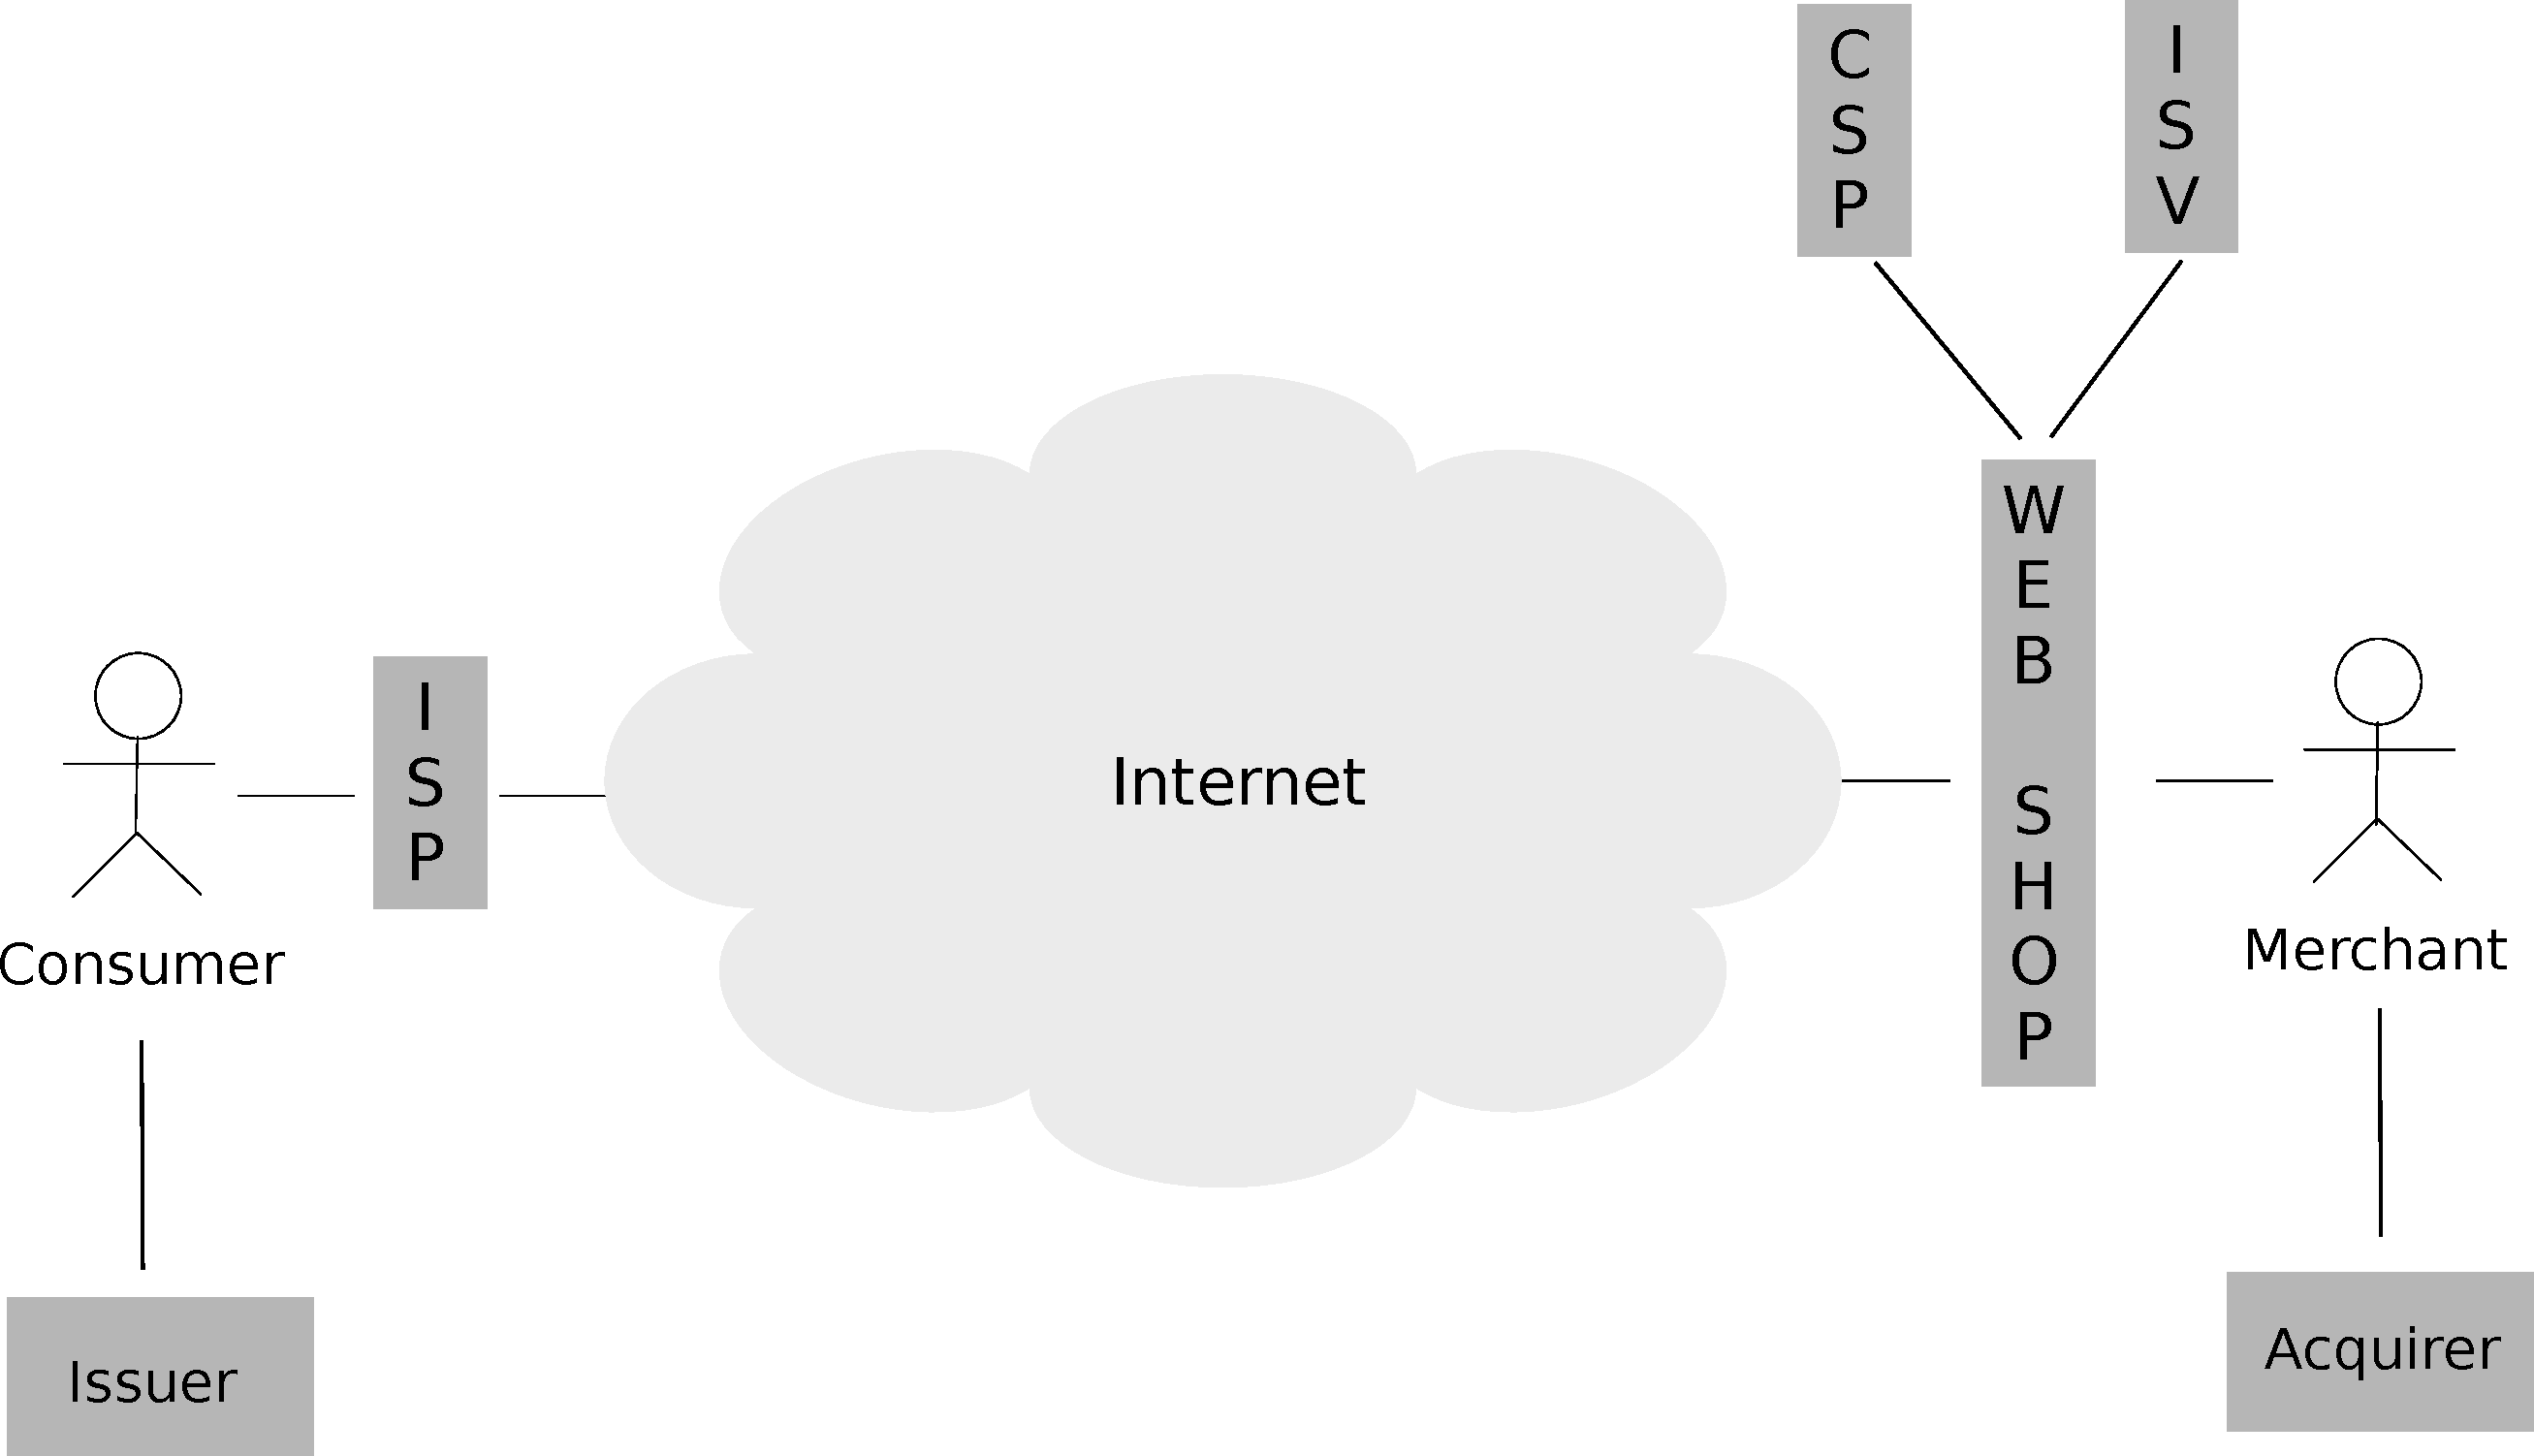
\includegraphics[width=0.8\columnwidth]{images/e-commerce-scenario.pdf}
	\caption{\gls{E-commerce} Fundamentals}
\label{fig:images_ecommerce_scenario}
\end{figure}

When the consumer places the order online, the merchant receives at least a list of products or services from the current shopping cart of the consumer, the identification of the consumer as well as the delivery address to ship the physical items to. If the transaction is going to be finalized with a credit card, the consumer will have to provide additional information like their billing address and credit card information (including the id, the expiry date and the security number of the card). \\

The merchants usually doe not validate the credit card information on their own. For that purpose they are relying on another 3$^{rd}$ party service offered on the Internet by the Payment Service Provider (\gls{PSP}). These providers are either validating the credit card information themselves based on an user profile the consumer has with the \gls{PSP} (e.g.\ a globally available Web service such as PayPal), or are connecting to the issuing bank of the credit card for doing so. For initiating this validation process the merchant is handing over the billing information to the \gls{PSP} incl.\ the credit card information given by the consumer. \\

Either the \gls{PSP} or the issuing bank is validating the correctness of these information with criterias like: \@

\begin{itemize}
    \item is the billing address matching the current consumers' postal address on file?
    \item is the stated credit card information correct?
    \item is the credit card still valid?
    \item is the credit card not marked as being blocked in the internal databases?
\end{itemize}

The merchant will receive the status of the authorization as well as an unique payment token in return. If the authorization was done successfully, the merchant will collect the items and send out a shipping request to one of the available Logistic Service Providers (\gls{LSP}), that are capable to handle the delivery of the order. They will pickup the items at the merchant's facility and ship them to the delivery address stated by the consumer. Usually in parallel the merchant is informing their bank about the order, amount due as well as the payment token received from the \gls{PSP}. The acquirer is in charge to withdrawal the amount of the order from the consumer's bank account either via the \gls{PSP} or directly from the issuing bank, depending on who of them has authorized the initial payment request (a process called clearing) \citep{VisaPayment2014}. The sequence of activities within an \gls{E-commerce} checkout process is visualized in Figure~\ref{fig:images_ecommerce_checkout_process}.\@

\begin{figure}[H]
	\centering
		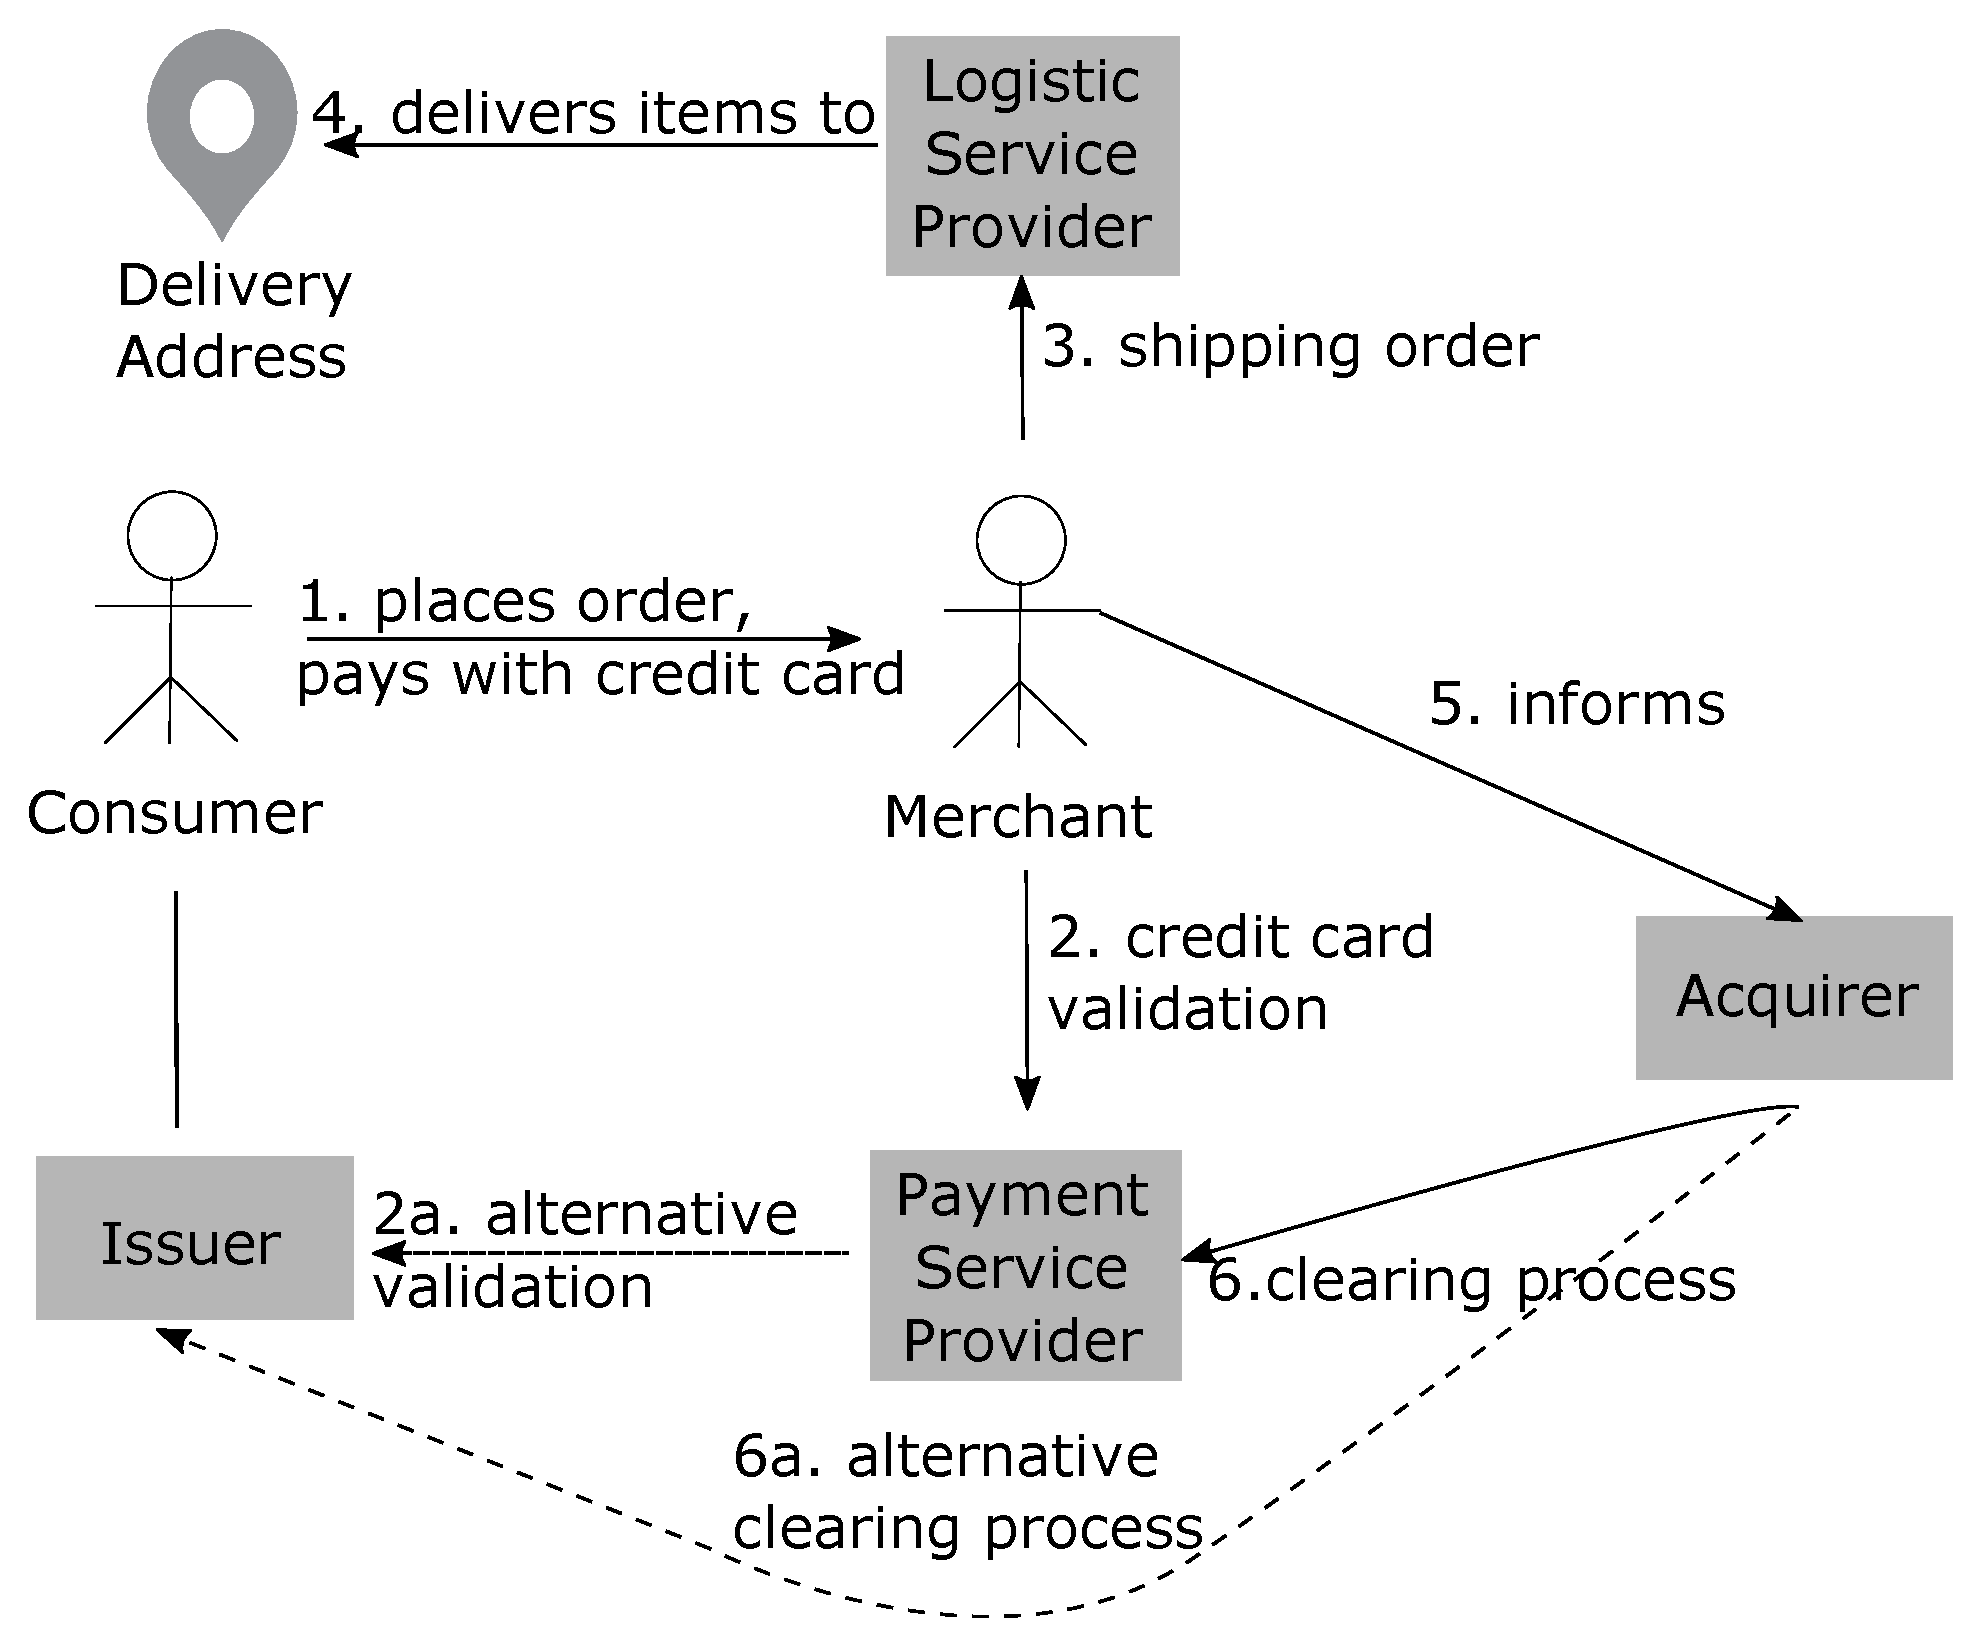
\includegraphics[width=0.8\columnwidth]{images/e-commerce-checkout-process.pdf}
	\caption{\gls{E-commerce} Checkout Process in detail}
\label{fig:images_ecommerce_checkout_process}
\end{figure}

% section scenario description (end)


% sub chapter stakeholder analysis
%!TEX root = ../MasterThesis.tex

\section{Stakeholders}
\label{sec:stakeholder_analysis}

The following section looks at each stakeholder involved in the E-commerce scenario in detail, lists the kind of information they own or provide to others as well as describes the role of each stakeholder in the E-commerce fraud investigation process (if any).

\subsection{Consumer}
\label{subsec:stakeholder_consumer}

The consumer is the initiator of an E-commerce transaction. She is using the shop of a merchant on the Internet to order products or services. For doing so she has to know the \gls{URL} of the Web shop, has to be connected to the Internet via the \gls{ISP} and has to use a standard software called a Web browser on her computer. For the duration of her online browsing session she also owns an unique \gls{IP} address handed out from the \gls{ISP}.\\

She might have had a long-term business relationship with the merchant and already owns an user account on the Web shop. On the other hand she might be just interested into a one-time shopping trip and might want to order the items without creating an account first --- sometimes also called ``anonymous checkout'' in the E-commerce shops. \\

The consumer is also having a bank account and at least owns a debit card with the issuing bank to get access to the money on that account. In addition to that she can also hold multipe credit cards. A credit card can be issued by the same bank or can be provided by another financial service (e.g. American Express). In any case the organisation that has handed out the credit card to the consumer is called the issuer. \\

If she is going to order items in a Web shop, she will usually browse the product and service offerings of the merchant first and put the items of interest into the shopping cart. When finalizing the transaction she has to state the following information to the merchant:\@

\begin{itemize}
		\item personal information incl.\ given name, family name and date of birth
		\item the address the items should be shipped to
		\item payment information incl.\ type of payment and billing address (if different to shipping address)
\end{itemize}

If she is going to end the transaction with a payment of type credit card she will also have to provide specific information of the card, that should be used for the payment:\@

\begin{itemize}
		\item the owner of the credit card (if it is not belonging to herself)
		\item the unique credit card number
		\item the expiry date of the credit card (in format MM/YY)
		\item the security code of the credit card
\end{itemize}

The consumer is having a special role in the whole scenario. As the online merchant has to deal with the consumer without any face-to-face or real-world interaction, the consumer is also the least thrustworthy party from the point of view of the merchant. As the Section~\ref{sec:scenario_fraud} will show, the consumer is the main object of question in the case of an E-commerce fraud incident. For the investigation of it the consumer is usually not taking any active part.

% subsection stakeholder consumer

\subsection{Merchant}
\label{subsec:stakeholder_merchant}

The merchant offers products and services on the Internet to the general public. She might use the Internet as an additional sales channel, or rely on it solely for making any business. To provide access to the Web shop the merchant has to register a domain name and an \gls{URL} with a local domain name registry. This specific \gls{URL} refers to a fixed public \gls{IP} address, that the server that runs the Web shop software uses. Normally the merchant does not operate the servers herself, but rely on a service offering from a hosting or cloud service provider for that. Also the Web shop software itself is usually not provided by the merchant, but bought from an \gls{ISV} on the market. In any case the merchant has special responsibilities in the Web shop, because she has to take care to configure the products, prices, promotions, payment and shipment services available. In addition products can be categorized by her into departments and sub-departments for easier navigating and searching the offerings in the Web shop by the consumer. \\

The merchant can decide whether she restricts ordering of products to registered users only, or allows anonymous users too. The main benefit of the former is the possibility to analyse the shopping behaviour of individual consumers, whereas the latter will open the business for a wider range of consumers as it includes also those, that do not want to register with any existing online shop. Nevertheless, any consumer activity on the online shop is tracked in the analytic databases of the merchant. This includes not only the items, that have been placed into the shopping cart, but also any product that has been looked at by the consumer during a shopping session. Even if these detailed analytic capabilities are actually synonymous for their usage in target-related advertising, they can also help to decide whether a consumer behaves normally or not. \\

Any business transaction that the consumer makes with the merchant is stored in the merchant's databases. A transaction information contains, but is not limited to:\@

\begin{itemize}
		\item the personal information of the consumer
		\item the address the items will be shipped to
		\item a collection of products with quantities and prices
		\item the total amount of the order considering promotions, taxes and fees
		\item the selected payment information
\end{itemize}

If the consumer pays with credit card, the merchant will not handle the payment herself, but relate this activity to a Payment Service Provider. To initiate the credit card authorization request, the merchant is sending the following information to the Web service endpoint of the \gls{PSP}: \@

\begin{itemize}
    \item consumer's billing address
    \item given credit card id, expiry date and security number
    \item identification of the merchant
    \item final amount of the current transaction
\end{itemize}

In return of the payment authorization the merchant will receive and store these  payment-related information for the transaction:\@

\begin{itemize}
		\item the type of credit card used (e.g. Visa, MasterCard, American Express, \ldots)
		\item the name of the credit card owner
		\item the payment token received by the \gls{PSP}
		\item the timestamp and result code of the authorization
		\item the authority who approved the payment (if the merchant works with multiple Payment Service Providers)
\end{itemize}

As a merchant will collect a lot of personal and payment-related information over time, she is also one of the major sources of possible data leaks in this scenario. Due to this circumstance the Payment Card Initiative, a group of banks, issuers and \gls{PSP}s, provides rules and guidelines (aka PCI/DSS standards) for securely handling these kinds of information in an IT system \citep{virtue2009payment}. \\

A merchant is one of the main actors in the fraud investigation process. She is highly interested in figuring out whether the consumer's transaction is valid or not. That is due to the fact, that in case of an E-commerce fraud incident the merchant will mostly have to cover the costs (see Section~\ref{sec:scenario_fraud}). Also the online merchant's reputation will suffer, if private information from her databases get leacked. If a merchant falls victim to a fraud incident multiple times, the economic damages can finally result in a bankruptcy of the merchant.

% subsection stakeholder merchant

\subsection{Payment Service Provider}
\label{subsec:stakeholder_psp}

The Payment Service Provider is offering payment-related services to online merchants. To be able to do this the \gls{PSP} provides a common Web interface, that the merchant has to communicate with for sending payment authorization requests (see above). The \gls{PSP} might be able to authorize the payment request on her own, or have to route the request to the corresponding issuer of the credit card in question. For the former procedure the \gls{PSP} has to run an own database of registered users with their credit card information (e.g.\ a Web service such as PayPal). For checking the credit card and authorizing the payment the merchant is sending the following information from the transaction:\@

\begin{itemize}
		\item credit card owner incl.\ billing address given
		\item credit card number
		\item credit card expiry date
		\item credit card security code
		\item identification of the merchant
		\item total amount of the current transaction
\end{itemize}

The \gls{PSP} has to securely process these information and return the result of the validation to the merchant. The result message also contains an unique payment token, that the merchant can refer to later to initiate the clearing process. As of this the \gls{PSP} has to persist the credit card and transaction-related information in her own backend databases. Following industry standards, she should do so according to the PCI/DSS guidelines mentioned in the previous section. \\

The level of activity in the E-commerce fraud investigation process depends on whether the \gls{PSP} authorizes the payment herself, or only acts as routing service between the merchant and the original credit card issuer. In the former case the \gls{PSP} is more actively involved. In that situation she also holds more of the valuable information to analyze the incident. In the latter case she will still be required to connect the payment-related request information from the merchant with the corresponding authorization result coming from the issuer.\\

If the \gls{PSP} holds sensitive information in her own databases, she will also be a source of possible data leaks. In that situation she has to put the same precautions in place as an issuing bank will have to do (see next section).

% subsection stakeholder psp

\subsection{Issuing Bank}
\label{subsec:stakeholder_issuer}

The issuer is one of the parties in the scenario that knows the owner of the credit card in person. Each individual has to register personally with the issuer to get access to a credit card. This registration process includes providing the following information: \@

\begin{itemize}
		\item personal information such as given name, family name and date of birth
		\item the currently registered home address
		\item the bank account that should be used to settle credit card balances
\end{itemize}

Even if the two parties do not really meet each other personally, an individual will still have to identify with a valid id card and bank account to receive and activate a new credit card. Beside being the single source of truth about the original credit card owner, the issuer of the card also collects and stores all  usages of it. The issuer therefore can provide individual credit card usage patterns, that are not just limited to the online shopping scenario --- something a Payment Service Provider can deliver too; but also include transactions the card owner does in the real-world. Needless to say that these are valuable information for the E-commerce fraud investigation. \\

Still the issuer does not know the details of the transactions, that have been made with the credit card yet. As shown in the Section~\ref{subsec:stakeholder_psp} the issuer will just receive an identifier of the merchant, in whose shop the credit card has been used. Based on public available information from a commercial register about the merchant, the issuer could at least come up with the retail branch the merchant operates in. \\

Being the single source of truth about all issued credit cards, their owners and usage patterns makes the issuer another high-risk participant for possible data leaks. She should as well follow the guidelines from the PCI/DSS standards, should incorporate security standards for her IT systems and processes as well as monitor her backend systems actively with an intrusion detection mechanism.

% subsection stakeholer issuer

\subsection{Acquiring Bank}
\label{subsec:stakeholder_acquirer}

The acquirer holds the bank account of the merchant and is responsible for withdrawing the outstanding amounts of transactions from the accounts of the consumers, or more precisely requesting it from the issuing bank of each consumer. As of this the acquiring bank is usually not processing any credit card related information from consumers, but refer to the payment tokens that have been given by the \gls{PSP} or issuer during the authorization process. \\

Still as a financial institute the acquirer (like the issuer) has to comply with the rules and guidelines of the PCI/DSS and other industry standards to make sure, that her bank accounts and the transaction processing are safe and secure. The detailed analysis of these techniques and procedures as well as possible banking fraud incidents are out of scope of this Master thesis though.

% subsection stakeholder acquirer

\subsection{Logistic Service Provider}
\label{subsec:stakeholder_lsp}

The Logistic Service Provider has two important roles in the E-commerce scenario. First, she has access to and control over the items of the merchant for the duration of the transport between the merchant's facility and the consumer's shipping address. And second, she holds the information to whom she has handed over the items at the final destination. Although the \gls{LSP} has nothing to do with any payment-related activities, she is still critical as she will be the last chance for the merchant to stop the delivery of the items (in case a fraud has been detected after initiating of the shipment), or provide information about the person that has received the items at the shipping address --- especially so on high-priced goods, that usually require the recipient to show her personal id card and place a signature on the delivery receipt. \\

For initiating the shipment procedure the merchant is ordering a certain transport service from the \gls{LSP} and hand over the following information:\@

\begin{itemize}
	\item name of the receiver
	\item delivery address given by the consumer
	\item list of items to be shipped
	\item optionally: value of the items if an insurance policy is taken
\end{itemize}

The \gls{LSP} at the other hand returns an unique tracking id for the shipment. It can be used by the merchant and the consumer to check the status of the shipment online. \\

As the \gls{LSP} does not have to deal with the payment-related activities in the E-commerce scenario, she is also not actively involved in the fraud investigation. Still she is of help, if an incident is found as she can stop the delivery or provide useful information about the recipient.

% subsection stakeholder lsp

\subsection{Cloud Service Provider}
\label{subsec:stakeholder_csp}

The Cloud Service Provider offers IT services to its customers. These IT services include hardware and software assets, that (in the E-commerce scenario) a merchant can order to run her Web shop on the Internet. Part of the service level agreement between the merchant and the \gls{CSP} is a detailed listing of the responsibilities of both parties (who has to take care of what). In most cases the merchant is outsourcing the complete operation of the hardware and software for the Web shop to the \gls{CSP}; so the \gls{CSP} will be responsible for making sure that the Web shop is accessible and secure. The \gls{CSP} is also constantly monitoring the incoming connections to each public Internet server under her control and can provide information, whether a Web shop of one of the merchants has been compromised or not.

% subsection stakeholder csp

\subsection{Independent Software Vendor}
\label{subsec:stakeholder_isv}

The \gls{ISV} designs, implements and sells the Web shop software. She has detailed knowledge about the software components and libraries used within the Web shop and checks them regularly for security breaches or vulnerabilities. She also has to verify the software code implemented on her own for vulnerabilities, and has to make sure that the implementation follows industry standards (e.g. PCI/DSS for handling person and payment-related information). Therefore she can best assert these quality criterias of the Web shop software if needed.

% subsection stakeholder isv

\subsection{Internet Service Provider}
\label{subsec:stakeholder_isp}

The \gls{ISP} provides a service to the consumer, so that she is able to connect to and use the Internet. Each Web request the consumer is doing on her system is routed to the public Internet via the infrastructure of the \gls{ISP}. Due to existing regulations and laws the \gls{ISP} has to store the log files of any Internet session of its customers for a certain amount of time. Especially, these log files can be helpful to decide whether a consumer was visiting pages in the dark-side of the Web, or if she falls victim to some phishing attacks (explained later in Section~\ref{sec:scenario_fraud}).

% subsection stakeholder isp

% section stakeholder analysis


% sub chapter data flow for credit card transactions
%!TEX root = ../MasterThesis.tex

\section{Data flow for credit card transactions}
\label{sec:stakeholder_data_flow}

As the previous chapter shows, there are a many stakeholders involved in providing \gls{IT} hardware, software and services to keep the Web shops on the Internet up and running. Only a small fraction of those will have to deal with the handling of credit card payments and order fulfillment though. These are the relevant stakeholders to look at in the case of an \gls{E-commerce} fraud incident. The actual flow of information between them is displayed in  Figure~\ref{fig:images_e_commerce_stakeholder}. \@

\begin{figure}[H]
	\centering
		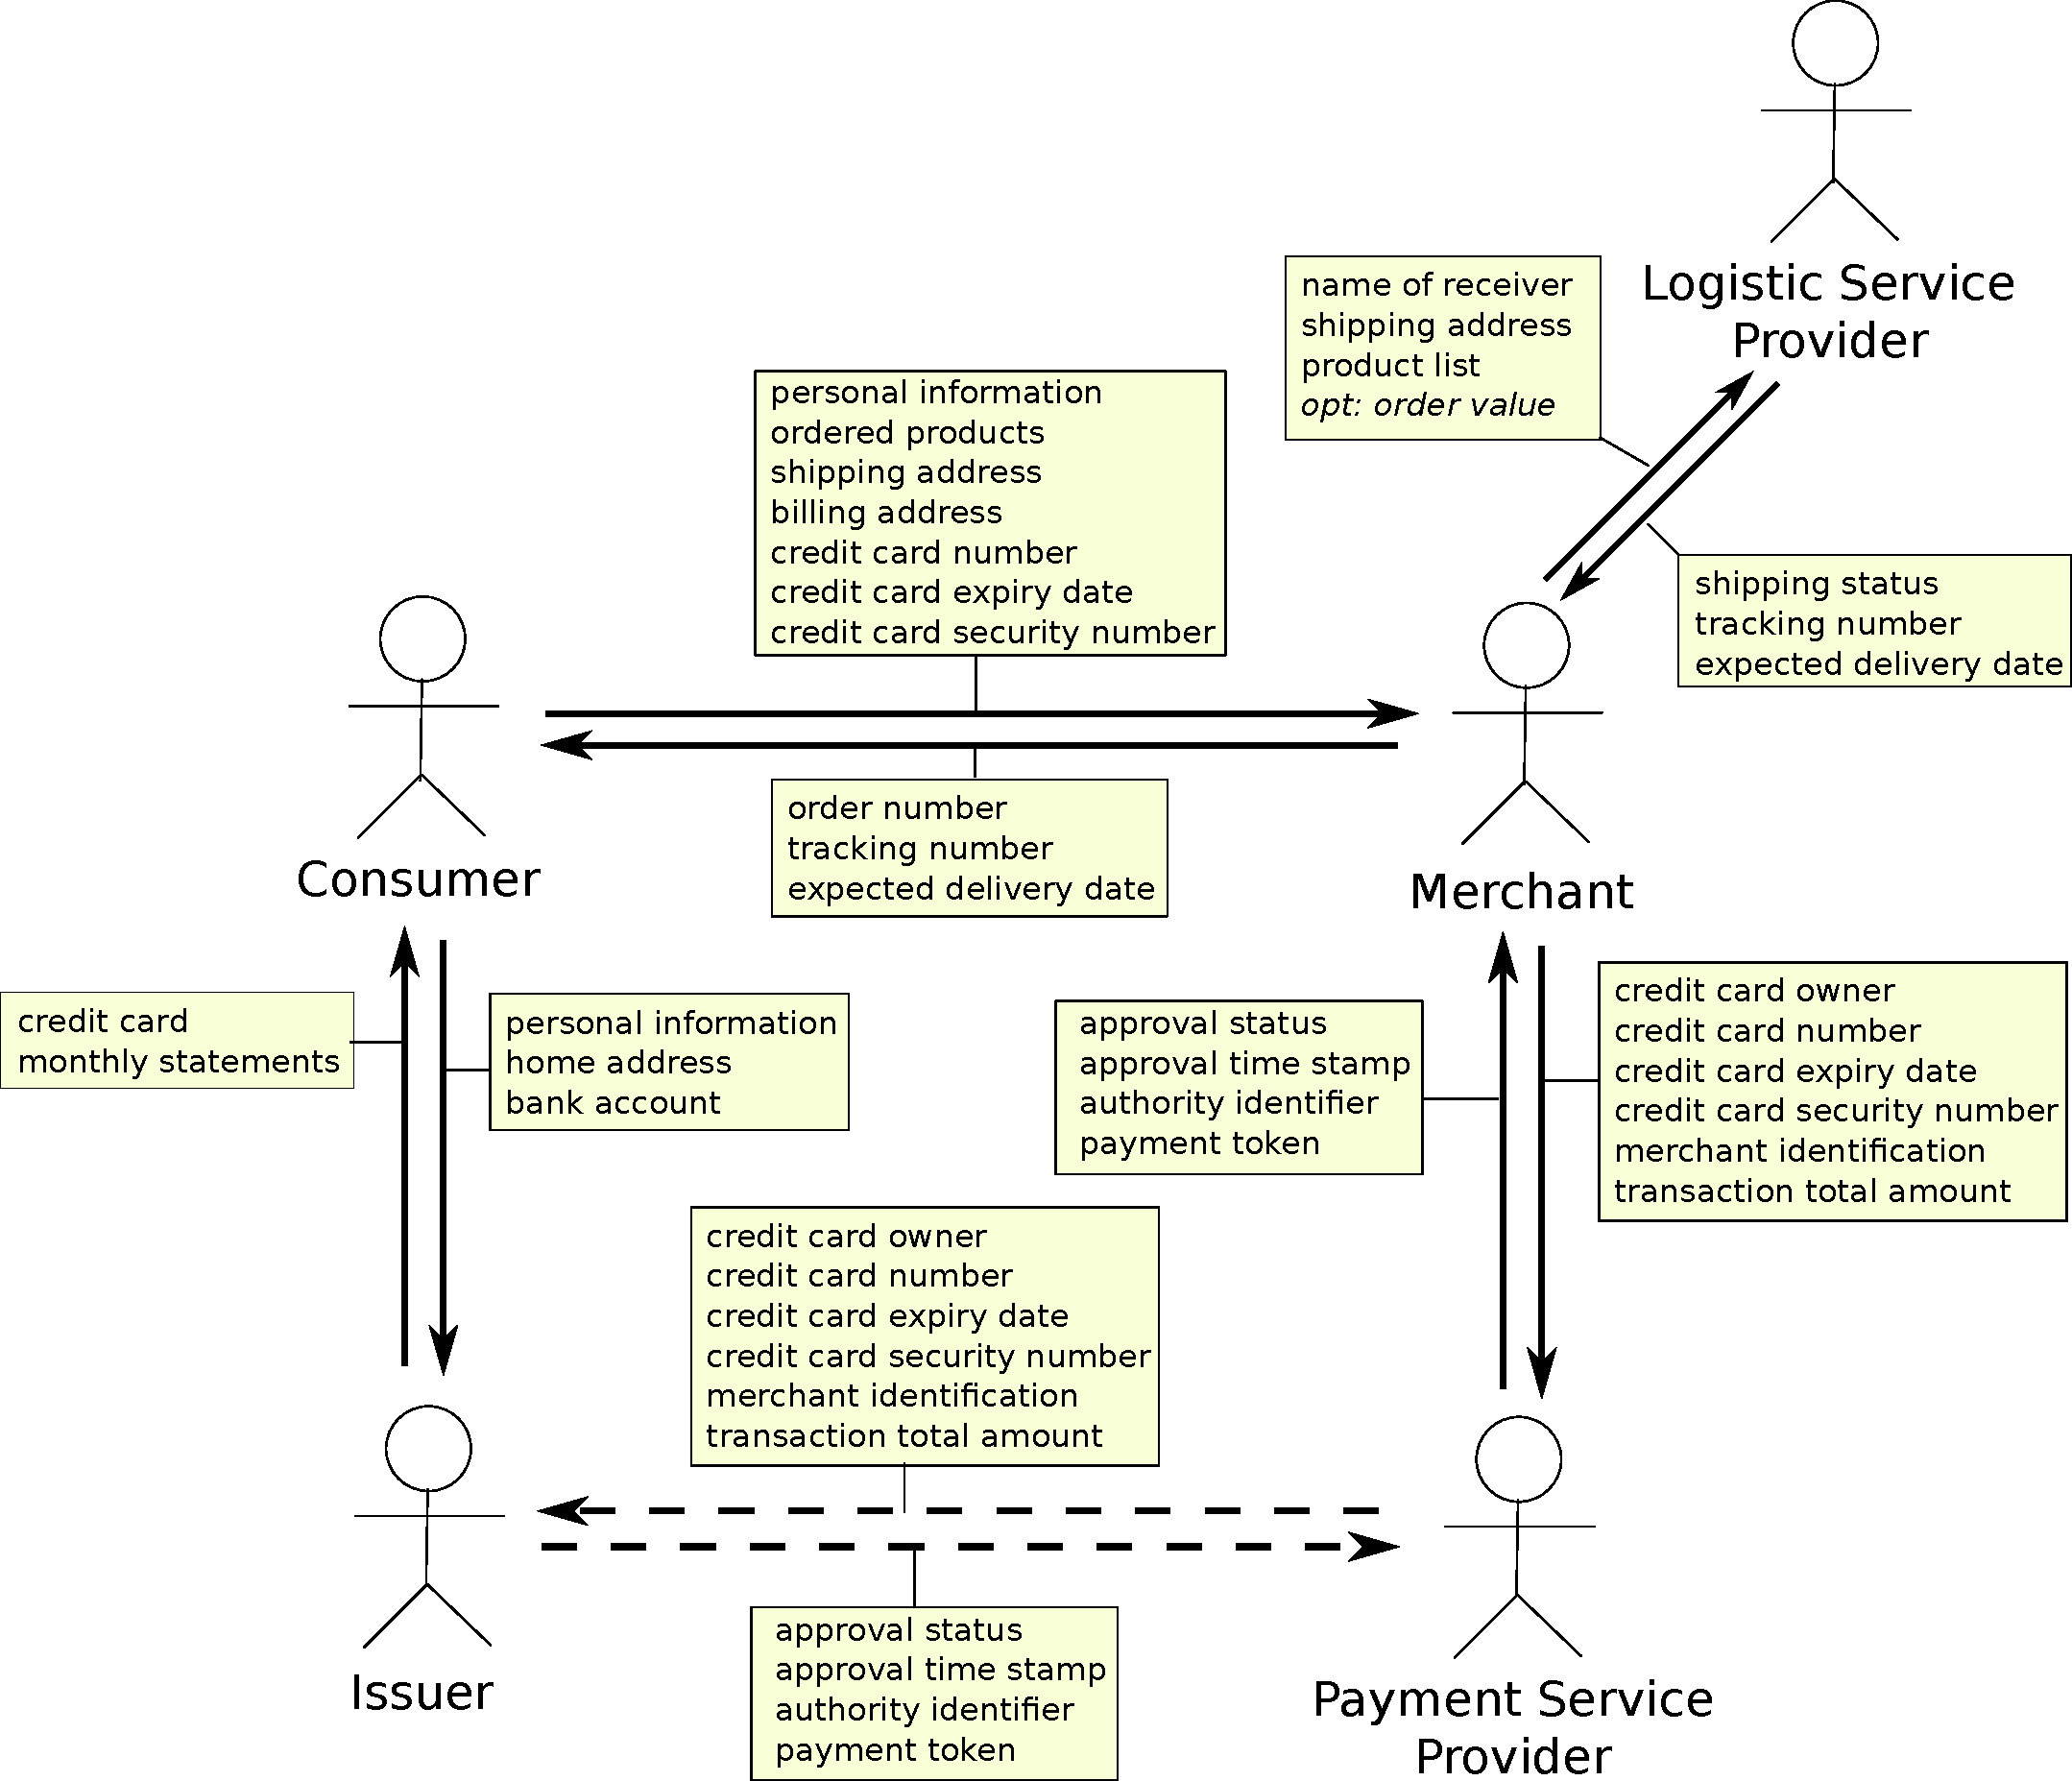
\includegraphics[width=0.8\columnwidth]{images/e-commerce-stakeholder.pdf}
	\caption{Stakeholder and Data Flow in \gls{E-commerce} scenario}
\label{fig:images_e_commerce_stakeholder}
\end{figure}


% sub chapter e-commerce fraud incidents
%!TEX root = ../MasterThesis.tex

\section{E-commerce fraud incidents}
\label{sec:scenario_fraud}

Based on the previous sections one can come up with strategies a fraudster might use to trick the E-commerce system. To do so the criminal will have to get access to credit card information in the first place. Therefore this section first looks into ways a criminal might get access to credit card and personal information in the E-commerce scenario. After that the section describes possible strategies a fraudster can use to trick the system. The section will end with a discussion of the E-commerce fraud incident handling as it is in place today.

\subsection{Credit Card data breaches}
\label{subsec:leaking_credit_cards}

 In the Section~\ref{sec:stakeholder_data_flow} one could already find the parties, who have access to or store credit card information in the E-commerce scenario, namely:\@

\begin{itemize}
  \item the consumer as owner of the credit card
  \item the issuing bank, who handed out the credit card to the consumer
  \item the merchant, if the consumer is paying with a credit card
  \item the Payment Service Provider, if the consumer is paying with a credit card online
\end{itemize}

The \textbf{\gls{PSP}} does receive the credit card information from the merchant during the authorization of the payment. If the \gls{PSP} does the authorization herself, she is also the party to store and hold the credit card information in her backend databases. As mentioned earlier the \gls{PSP} should follow industry standards and guidelines for storing and processing payment related information, especially the PCI/DSS standard. Also she is responsible for monitoring her systems with an intrusion detection program. This will trigger a signal as soon as an hacker got access to the internal databases. In that case the \gls{PSP} can put the leaked credit card information on an internal blacklist, so that these cards could no longer be used for further payments online. Additionally she will have to send a message to the affected issuers, to which the \gls{PSP} generally maintains a strong business relationship. The issuer will inform the affected owners and send out new credit cards to them. Due to this procedure in place, one can assume that the safety and security of credit card handling at the \gls{PSP} can be guaranteed. \\

The \textbf{merchant} receives the credit card information during the checkout process from the consumer. The credit card information is transfered via the public Internet from the consumer to the merchant and could be a victim of a man-in-the-middle attack, in which the hacker is intercepting the communication between the consumer and the merchant with the objective to capture the personal and payment-related information from the data transmission stream. Therefore the merchant should offer the Web shop only via a secure connection using industry standards like TLS to encrypt the information send between both parties. This will make it more difficult for an attacker to get to the plaintext information exchanged between consumer and merchant. \\

As the merchant is not processing the credit card information directly, she also do not have to store them in her own backend databases. The merchant is asking the \gls{PSP} or issuer of the card for authorization of the credit card payment and receives an \textbf{unique payment token} in response, if the authorization was successful. As stated in the PCI/DSS standard a merchant should never store the whole credit card data, but should use this payment token and shortened credit card information (especially abbreviated credit card numbers) to refer to the single payment later. Due to this one can conclude, that breaking into the systems of a merchant will not result in any leaked credit card information, if the merchant follows these PCI/DSS standards. \\

The \textbf{issuer} is a valuable target for hacking into the backend systems with the objective to leak a massive amount of credit card and owner information. As a financial institute the issuer have to follow a huge set of regulations and safety procedures to be able to participate on the market. It can be assumed that at least the same safety mechanisms are valid as for the \gls{PSP} are in place. This means constantly monitoring the internal systems with an intrusion detection mechanism and blacklisting any leaked credit card. In addition to the monitoring of all online activities (as also the \gls{PSP} does) the issuing bank can monitor activities done with the credit card in the offline world too. In case of suspicious activities the credit card can be blocked and a new one will be send out to the credit card owner. \\

The \textbf{consumer} is also a valuable target for eavesdropping on credit card and personal information. She is also the weakest and most unsecure party in the whole E-commerce scenario. As said above a lot of the protection mechanisms of the other parties are relying on implementing industry standards and on constantly monitoring the own systems for malicious activities. This can not be securely said about the computer of the consumer. Whether she is using up-to-date security programs (e.g.\ an Antivirus tool and a firewall) on her computer or not is out of reach of the other parties to verify. Additionally a consumer can fall victim to a phishing attack, that will send her to a malicious Web site with the intend to get her personal information. In some seldom cases the consumer might cooperate with the fraudster or might be the fraudster itself with the intend to trick the system for her own interest. As of this the E-commerce fraud investigation can not rely on information from the consumer, but instead has to figure out, if the transaction in question was made from the real owner of the credit card or from a frauster.

% subsection leaking_credit_cards (end)

\subsection{E-commerce fraud strategies}
\label{subsec:strategies_fraudster}

After a fraudster has got access to leaked credit card information she can come up with the following strategies to trick the E-commerce system:\@

\begin{enumerate}
  \item a fraudster owns \textbf{one} leaked credit card information and try to use it for ordering products from \textbf{multiple} merchants on the Internet
  \item a fraudster owns \textbf{multiple} leaked credit card information and try to use them for ordering products from \textbf{one} merchant on the Internet
  \item a combination of the two cases mentioned before, that can also be related to as a series of the first fraud activity
\end{enumerate}

In the \textbf{first scenario}, in which the fraudster is trying out a leaked credit card for ordering products on Web shops of various merchants online, each of the merchant only sees the transaction that takes place in her system. It will make it more difficult for the merchant to decide whether this is a fraud transaction or not, as she is not aware of the attempts the fraudster has done on other merchant's Web shops. \\

As each merchant will rely on a \gls{PSP} or issuer to verify the credit card payment, it is in the responsibility of these parties to recognize fraud transactions in this scenario. To be able to do this the \gls{PSP} and also the issuer are monitoring the usage of credit cards and are actively looking for suspicious activities. The fraud prevention mechanisms in place are mostly working on a rule-based, and in some cases also score-based systems running in the internal network of the \gls{PSP} and issuer. These systems are fed with the information the merchant sends with the payment authorization request and will come up with either:\@

\begin{enumerate}
  \item Yes, this looks like a fraudulent transaction and will be blocked
  \item No, this seems to be a valid transaction and will be acknowledged
  \item Maybe, this transaction might be valid, but there is some uncertainty in the validation of it. These edge cases are routed to a human operator of the \gls{PSP} or issuer to decide on how to proceed with it
\end{enumerate}

As a recent study shows the success rate of the fraud prevention systems heavily relies on the techniques used to validate the transaction data \citep{rana2015survey}. The outcome is, that ca. 70 to 80 percent of the fraudulent transactions will be recognized as such and blocked successfully. That still means 20 to 30 percent of fraudulent transactions could not be recognized as such. For handling these cases the organisations employ special trained staff, that is operating 24/7 and 365 days a year. \\

As stated in the introduction of this Master thesis there is a shift from the offline credit card fraud to the online world. This is also resembled in current figures of E-commerce frauds, whose show that it makes up ca. 85 percent of all credit card fraud attempts and have on average a transaction amount of 500 to 600 EURO.\\

As the \gls{PSP}s and the issuers do not have any order details, they can only decide on the information given during the authorization request (see Section~\ref{sec:stakeholder_analysis}). At most they can validate the branch the merchant is operating in, and it might come as no surprise that the fraudsters are regularly using Web shops of merchants, who offer either electronics, clothings, entertainment- or travel-related products. These are also the most commonly used sources of \textbf{\underline{valid}} E-commerce transactions and therefore make any fraudulent transaction very difficult to detect. \\

At the end it might be the owner of the credit card, who detects suspicious activities on her credit card account and informs the issuing bank about it. Based on current regulations and laws the issuing bank has to rollback the fraudulent transaction on request of the consumer, which means that the merchant will have to cover the costs of the E-commerce fraud (as she is not receiving the money for the products that has been already shipped to the fraudster). \\

Looking at the \textbf{second scenario} of the E-commerce fraud strategies at the beginning of this section, a merchant will receive multiple requests from a fraudster, who is trying out various leaked credit cards for finishing an order process. This kind of E-commerce fraud can be recognized at the systems of the merchant based on the same source \gls{IP} address of the requests or due to having the same shipping address for orders with different credit cards. Due to that one can conclude, that also merchants must take an active role in the fraud prevention process (if they do not do so already) and try to minimize the amount of fraudulent transactions taken place on their Web shops. As this scenario is likely be manageable with additional fraud prevention mechanisms at the merchant without the need to involve other parties of the E-commerce scenario, this second scenario falls out of scope of this Master thesis.

% subsection strategies_fraudster (end)

\subsection{E-commerce fraud incidents handling}
\label{subsec:e_commerce_fraud_handling}

If the fraud prevention systems at the \gls{PSP} or issuer are detecting a suspecious transaction an operator of a special department within the organisation will be informed about the transaction via a notification on his computer. This operator will have to decide if the transaction looks valid and should be acknowledged or seems to be fraudulent and has to be denied. To be able to decide this she is going to look into the usages of the credit card in question for the near past. Whereas it will be easy to recognize that a credit card, that was just being used in a shop in Germany could not be used in a shop in US or Asia within a short timeframe due to physical constraints in the real world, the same consumer can order products from an US or Asian online retailer with ease within minutes. So these initial geographical contraints, that work well with real world usage patterns of credit cards (a strategy called geo-fencing), will no longer work in the E-commerce scenario. \\

So the operator has to found her decision on the transaction information at hand. Initially she can check for the amount that should be paid with credit card. One can assume that small amounts will be covered by the \gls{PSP} or issuer, who will take over the risk for a false authorization. With an increased value of the items ordered the \gls{PSP} or issuer is putting back the risk to the merchant in case of a customer complaint later. At a second glance she can verify whether the consumer has had any business relationship with the merchant in the past as well as validate the retail branch the merchant operates in. Though these are weak hints for investigating the validity of an E-commerce transaction (see above). \\

To make a solid decision the operator will have to get in contact with the merchants the credit card has been used with recently and ask for additional information like:\@

\begin{itemize}
  \item does the consumer owns an user account with the Web shop?
  \item does the shipping address matches the billing address for the order?
  \item if not has the user ordered products to this shipping address in the past?
  \item what has been ordered, incl.\ detailed product information like brand, model, product categories, \ldots
\end{itemize}

In some cases the \gls{PSP} or issuer might have had a business relationship with the online merchant in the past and already knows the support personell from the merchant to contact for querying, but in most cases the contact person might not be known to the \gls{PSP} or issuer resulting in asking the general support via the contact formulars on the merchants Web site. \\

Executing this procedure with multiple online merchants from different countries will be time consuming and raise a lot of efforts at the \gls{PSP}s, issuers and merchants. Getting the right information might take time as the correct addressee from the support department of the merchant is unknown, the merchant do not have specialized staff at hand to handle these kind of issues, or there are misunderstandings on handling the case due to language barriers or different incentives. Therefore one can assume that this detailed analysis of any suspecious transaction will not take place today, but most of these transactions will be acknowledged after a first short look at them. \\

Still the merchants as well as the \gls{PSP} and issuer have a high incentive for keeping the success rate and numbers of these fraudulent activities low. For the \gls{PSP} and issuing bank there are regulations stating that at maximum only 1 thousands of the overall transactions (numbers for the EU) should be fraudulent. This keeps the pressure on these financial instituts to invest in fraud prevention techniques for being able to stay in business. For the merchant it is of high interest that a fraudulent transaction can be resolved before the fraudster receives the ordered products. In the worst case scenario of just one successful fraudulent transaction in an E-commerce shop, past experience shows that this will trigger hundreds if not thousands of following attempts from other fraudsters. \\

% subsection e_commerce_fraud_handling

% section scenario_fraud (end)


% sub chapter scope of thesis
%!TEX root = ../MasterThesis.tex

\section{Scope of this Master Thesis}
\label{sec:scope_thesis}

As laid out in the previous section, the most interesting E-commerce fraud scenario is the one, in which a fraudster uses a leaked credit card information to order products or services from various merchants on the Internet. This is currently most likely to be successful, because there is a lack of information on the side of the merchant as well as the \gls{PSP} or issuer. Each of the affected merchants just noticed the single transaction that takes place on her own Web shop, without knowing about the other attempts the fraudster do on other Web shops. The \gls{PSP} and issuer will notice the active use of the credit card on different Web shops though, but do not have any information about the transaction details. Therefore they could not correlate these information to check for suspicious activities. \\

Based on the current credit card usage patterns of the fraudsters, whose will use a leaked credit card information in commonly used Web shops, which deal with electronics, entertainment or travel-related products and services, it is more likely that these fraudulent transactions will not be recognized on time by the existing fraud prevention mechanisms in place today. \\

A simple approach to solve this issue would be to just share more information of the ongoing transaction between the merchants, the \gls{PSP}s and the issuers. This might be subject to fail though, because each party has to follow the restrictions and regulations for sharing personal-related information. Additionally adapting and harmonizing the communication interfaces between the Web shops from various online merchants and the Web interfaces of different \gls{PSP}s and issuers are an enormous undertaking and will likely not succeed due to different notions of the communication patterns and data structures exchanged between all relevant participants. \\

This shows the scenario this Master thesis will look into in detail and try to solve the most important question: \textit{is this really a fraudulent transaction?} \\

Looking into the stakeholders, that can provide useful information to decide on it, one will come up with:\@

\begin{enumerate}
    \item \textbf{merchant}, who can provide additional information of each E-commerce transaction in question
    \item \textbf{\gls{PSP}/issuer}, whose offer information about the credit card usage pattern and the original credit card owner
    \item \textbf{\gls{LSP}}, who can offer information about whether the order has already been shipped or not, and in the former case to whom it has been handed over
    \item \textbf{\gls{ISP}}, who can on request give hints whether a consumer has fallen victim to a phishing attack based on her Internet access logs
\end{enumerate}

% section scope_thesis (end)


% chapter context analysis (end)
